\chapter{Methods}\label{chap:methods}
\fancyhead[LO]{\nouppercase{\leftmark}}

\section{Modelling smooth latent dynamics within a VAE framework}\label{sec:methods-generalintro}

We have seen that VAEs can infer lower-dimensional representations of the central factors of variation in a dataset. In the simulated data setting outlined in Chapter~\ref{chap:intro}, we have such an underlying low-dimensional dynamical system from which the observations are generated.
In an epidemiological cohort study such as the NAKO, we are typically interested in the underlying concept of the study participants' general condition and their mental and physical health status and try to access that health status, being a complex phenotype, by taking a multitude of individual measurements. It is thus plausible to assume the presence of groups of variables that jointly describe a more general underlying concept, e.g., we can imagine to collect data on individual's BMI, frequency of physical acticity, resting pulse rate and dietary habits all contributing to a latent representation of the individual's general physical fitness. 
Since we do not know specifically in what way single variables contribute to which part of a latent structure, the VAE provides a viable tool to infer such a latent representation directly from data in an unsupervised way, allowing for potentially complex, non-linear interactions. My model to infer the underlying lower-dimensional development patterns is therefore based on a VAE architecture.

The data are viewed as snapshots from a process evolving continuously over time that is observed with measurement noise. Consequently, also the underlying latent structure can be assumed to consist of dynamics changing smoothly over time and the latent space-representation has to be constrained to describe such smooth temporal development patterns. In my model, I formulate this constraint as the assumption that the latent space can be described by a system of differential equations that capture the basic dynamics underlying the observations.
This implies that the latent variable $Z$ should represent both a random variable and a function changing over time, i.e., a stochastic process.
Regarding the elements of stochasticity in the observed process, I assume a "true", inherently deterministic underlying dynamic process and a random force not acting on the process itself, but on a noisy observation of it. That observation is governed by some level of uncertainty, which I assume to be independent of the observation time. 
As a result, the latent space of the VAE model should encode a low-dimensional representation of the data that matches a smooth trajectory, with a stochastic element accounting for the uncertainty in the generating process of observations from an inherently deterministic underlying trajectory. 
This implies to model the stochasticity of the process as the random measurement error in the observations that can be assumed to be distributed according to $\mathcal{N}(0,\sigma^2)$. 
Consequently, I employ a Gaussian prior and posterior for the latent random variable $Z$. Here, the posterior mean represents its value according to the deterministic trajectory described by the ODE system, while the variance accounts for the uncertainty in the observation of that value. 

Summing up, I describe the true deterministic process from which data are generated as an ODE system imposed on the latent space formulated in terms of the posterior mean $\mu_{\mathrm{post}}$ of $\Q^{Z\mid x} = \mathcal{N}(\mu_{\mathrm{post}}, \sigma_{\mathrm{post}}^2)$ to account for the assumption of modelling a deterministic process with a random element in its observation, but not the temporal development itself. I therefore constrain the latent space to describe smooth dynamics by solving an ODE system for the posterior mean. To model the stochasticity of the measurement process, I subsequently sample $z$ from the posterior distribution according to smooth dynamics after solving the ODE and decode it to the data space to obtain a reconstructed observation.

\section{Fitting individual ODE parameters with baseline variables}\label{sec:methods-ODEparamswithbaselineinfo}

As a further important feature, the model should be capable of extracting individual-specific development patterns, i.e., to fit individual ODE systems to the posterior mean of the latent representation. Since this representation should recover the main factors of variation that govern the observed developments, I define a low-dimensional system of ODEs with one equation for every dimension of the latent representation that can be thought of as an underlying common trend shared by several variables in the original dataset.  

The general structure of the ODE is explicitly specified as a linear system in Chapter~\ref{chap:applications}, Sections~\ref{sec:apps-linear2p} and \ref{sec:apps-linear4p} or as a non-linear system in Chapter~\ref{chap:applications}, Section~\ref{sec:apps-nonlinear2p}, but the parameters of the pre-defined system are determined individually for each input observation to account for different development patterns in the same set of measured variables.
To infer such an individual-specific set of ODE parameters, I employ the additional variables measured only at the baseline timepoint, assuming that this more extensive characterisation carries information about each individual's development. 
Since I assume it to be unknown how they specifically relate to the individual ODE parameters, I employ an additional neural network to map the observations of the baseline variable to a set of ODE parameters for each individual. I train this network jointly with the VAE model, since the model should find a latent representation matching the assumption that the latent space can be described by an ODE system. By training jointly, the ODE structure imposed on the latent space is allowed to influence the VAE training and guide the model to find an appropriate latent representation.

As an example to motivate this method, we can imagine to measure several time-dependent variables describing lung function and at baseline also collect information about chronic lung diseases, age, physical activity and smoking habits. Then, these additional baseline measurements can potentially be informative about the development of each individual's lung function. More generally, if there are groups of individuals sharing common development trends, e.g., chain smokers, the baseline variables could contain information from which an individual's group membership can be deduced. 

\section{Derivation of the ODE-VAE training objective}\label{sec:methods-ODE-VAEtraining}

I now formalise my method by describing the training process of the model and deriving an adapted version of the ELBO to define the loss function. 

The dataset $\mathcal{D} = \lbrace x_1,\dots, x_n\rbrace$ includes $n$ observations that each consist of two measurements of $p$ variables, i.e. $x_i = (x_i\tn \quad x_i\te) \in \R^{p\times 2}$ with $x_i^{t_j}= (x_{i,1}^{t_j}, \dots, x_{i,p}^{t_j})^{\top} \in \R^{p}$ for $j=0,1$.
The encoder part of the VAE maps an input observation $x_i$ column-wise to the mean  $\mu_i= (\mu_i\tn \quad \mu_i\te) \in \R^{k\times 2}$ and standard deviation $\sigma_i = (\sigma_i\tn \quad \sigma_i\te) \in \R^{k\times 2}$ of the posterior distribution $\mathbb{Q}^{Z\mid x_i} = \mathcal{N}(\mu_i,\sigma_i^2)$, where $k$ is the dimension of the latent space.

For each individual $i$, I denote with $y_{i,1},\dots, y_{i,q}$ the measurements of the additional baseline variables used to infer the parameters of the ODE system in latent space. A neural network that I refer to as the \textbf{ODE-net} maps the corresponding observation $y_i = (y_{i,1}, \dots, y_{i,q})^{\top} \in \R^q$ to a set of individual ODE parameters $\eta_i \in \mathbb{R}^l$, with $l$ being the number of parameters of the ODE system. 

The latent space dynamics are given by a pre-specified function $f(\mu_i(t), t, \eta_i)$ that describes either a homogeneous two-dimensional linear ODE system or a non-linear Lotka-Volterra ODE system. 
The parameters of this ODE system are inferred from the individual-specific baseline measurements with the ODE-net.
Then, we can solve the initial value problem 
\begin{equation*}
\begin{split}
	\frac{d}{dt} \mu_i(t) &= f(\mu_i(t), t, \eta_i)\\
	\mu_i(t_0) &= \mu_i\tn
\end{split}
\end{equation*}
at $t_i^{1}$, the time point of the individual's second measurement, and obtain a vector $\widetilde{\mu_i}\te = \mathrm{ODESolve}(f(\mu_i(t), t, \eta_i), \mu_i\tn, t_i^{1}) \in \R^k$. We now define $\widetilde{\mu_i} := (\mu_i\tn \quad \widetilde{\mu_i}\te)$ as the mean of the posterior distribution constrained to a smooth dynamic and draw a sample $z_i\sim \widetilde{\Q}^{Z\mid x_i}_{\eta_i,\phi} = \mathcal{N}(\widetilde{\mu_i}, \sigma_i^2)$ from the approximate posterior. Subsequently, $z_i$ is passed to the decoder of the VAE that parameterises $P_{\theta}^{X\mid z_i}$, the conditional distribution of the data given a sample of the posterior, to obtain a reconstructed observation $\widehat{x_i}$ as a sample from $P_{\theta}^{X\mid z_i}$. 

To define a training objective for jointly optimising the VAE model constrained to smooth latent space dynamics and the ODE-net, I adapt the ELBO of (\ref{elbo-as-function-of-theta-and-phi}): To learn the latent space dynamics according to the ODE system jointly with the network supplying the parameters of this system, the posterior mean as obtained from solving the ODE is used. Because this mean and therefore also the posterior distribution depends on the parameters $\eta_i$ of the individual's ODE system, we thereby introduce dependence of the ELBO on the ODE parameters and hence provide feedback for learning the weights and biases of the ODE-net:
\begin{equation}
\begin{split}
\mathrm{ELBO}_{\mathrm{smooth}}(x_i\tn, x_i\te, \eta_i, \theta, \phi) &= -D_{\mathrm{KL}}(\widetilde{q}_{Z\mid x_i\tn, x_i\te}(\cdot, \eta_i, \phi) \Vert p_Z(\cdot,\theta)) \\ 
&+ \E_{\widetilde{q}}[\log(p_{X\mid z_i\tn, z_i\te}(x_i\tn, x_i\te,\theta))],
\end{split}
\end{equation}
where $\widetilde{q}$ is used as an abbreviation for $\widetilde{q}_{Z\mid x_i\tn, x_i\te}(\cdot, \eta_i, \phi)$ in the expectation.
Since the solution of an ODE is uniquely defined (if it exists) by the function specifying the derivative and the initial value according to Theorem~\ref{thm:picard-lindelöf} (Picard-Lindelöf), the ODE solution $\widetilde{\mu_i}\te$ depends exclusively on the initial value $\mu_i\tn$ and the ODE parameters $\eta_i$, but not on the observations at the second time point $x_i\te$. 
It follows that the posterior distribution $\widetilde{\Q}^{Z\mid x_i}_{\eta_i, \phi}$ is independent of $x_i\te$, hence $\widetilde{q}_{Z\mid x_i\tn, x_i\te}(\cdot, \eta_i, \phi) = \widetilde{q}_{Z\mid x_i\tn}(\cdot, \eta_i, \phi)$. To improve the capability of the model to still reconstruct $x_i\te$ along with $x_i\tn$ and to provide feedback for the encoder weights and biases with respect to $x_i\te$, the loss is augmented with the squared euclidean distance between $\mu_i\te$ as obtained from directly passing $x_i\te$ through the encoder and $\widetilde{\mu_i}\te$ as obtained from solving the ODE.
By minimising that distance, the posterior distribution from the encoder $q_{Z\mid x_i\tn, x_i\te}(\cdot,\phi)$ is brought to match the posterior distribution $\widetilde{q}_{Z\mid x_i\tn}(\cdot, \eta_i, \phi)$ constrained to smooth latent space dynamics. In that way, the model is encouraged to encode the data from both measurement time points into a lower-dimensional representation that matches the smooth structure reinforced by the ODE system even before applying the ODE solving step.
Since the encoder posterior $q_{Z\mid x_i\tn, x_i\te}(\cdot,\phi)$ directly depends on $x_i\te$, bringing it close to $\widetilde{q}_{Z\mid x_i\tn}(\cdot, \eta_i, \phi)$ implicitly provides feedback from $x_i\te$ on $\widetilde{\mu_i}\te$ and thus achieves an implicit conditioning of $\widetilde{q}_{Z\mid x_i\tn}(\cdot, \eta_i, \phi)$ on $x_i\te$. Adding the term with a weighting factor of $\alpha\in[0,1]$ results in the final loss
\begin{equation} \label{finalELBO}
\begin{split}
\mathcal{L}(x_i\tn, x_i\te, \eta_i, \theta, \phi) &= -\mathrm{ELBO}_{\mathrm{smooth}}(x_i\tn, x_i\te, \eta_i, \theta, \phi) + \alpha\Vert\mu_i\te - \widetilde{\mu_i}\te\Vert_2^2 \\
=&\dkl(\widetilde{q}_{Z\mid x_i\tn, x_i\te}(\cdot, \eta_i, \phi) \Vert p_Z(\cdot,\theta)) \\
&- \E_{\widetilde{q}}[\log(p_{X\mid z_i\tn, z_i\te}(x_i\tn, x_i\te,\theta))]\\
&+ \alpha\Vert\mu_i\te - \widetilde{\mu_i}\te)\Vert_2^2.
\end{split}
\end{equation}

Note that by minimising $\mathcal{L}$, we still maximise a lower bound on the data likelihood, since the negative loss equals the ELBO with a positive term subtracted. Heuristically, by jointly maximising the ELBO and minimising the distance of $\mu_i\te$ and $\widetilde{\mu_i}\te$ via minimising $\mathcal{L}$, we can even obtain a lower bound closer to the true data likelihood due to the implicit conditioning of the smooth posterior $\widetilde{\Q}_{\eta_i, \phi}$ on $x_i\te$, which potentially leads to a better reconstruction error while still maintaining a smooth dynamic structure of the latent state. 
Figure~\ref{fig:node_vae_architecture_draft} provides a graphical overview of my model and its training process. 

\begin{figure}[H]
	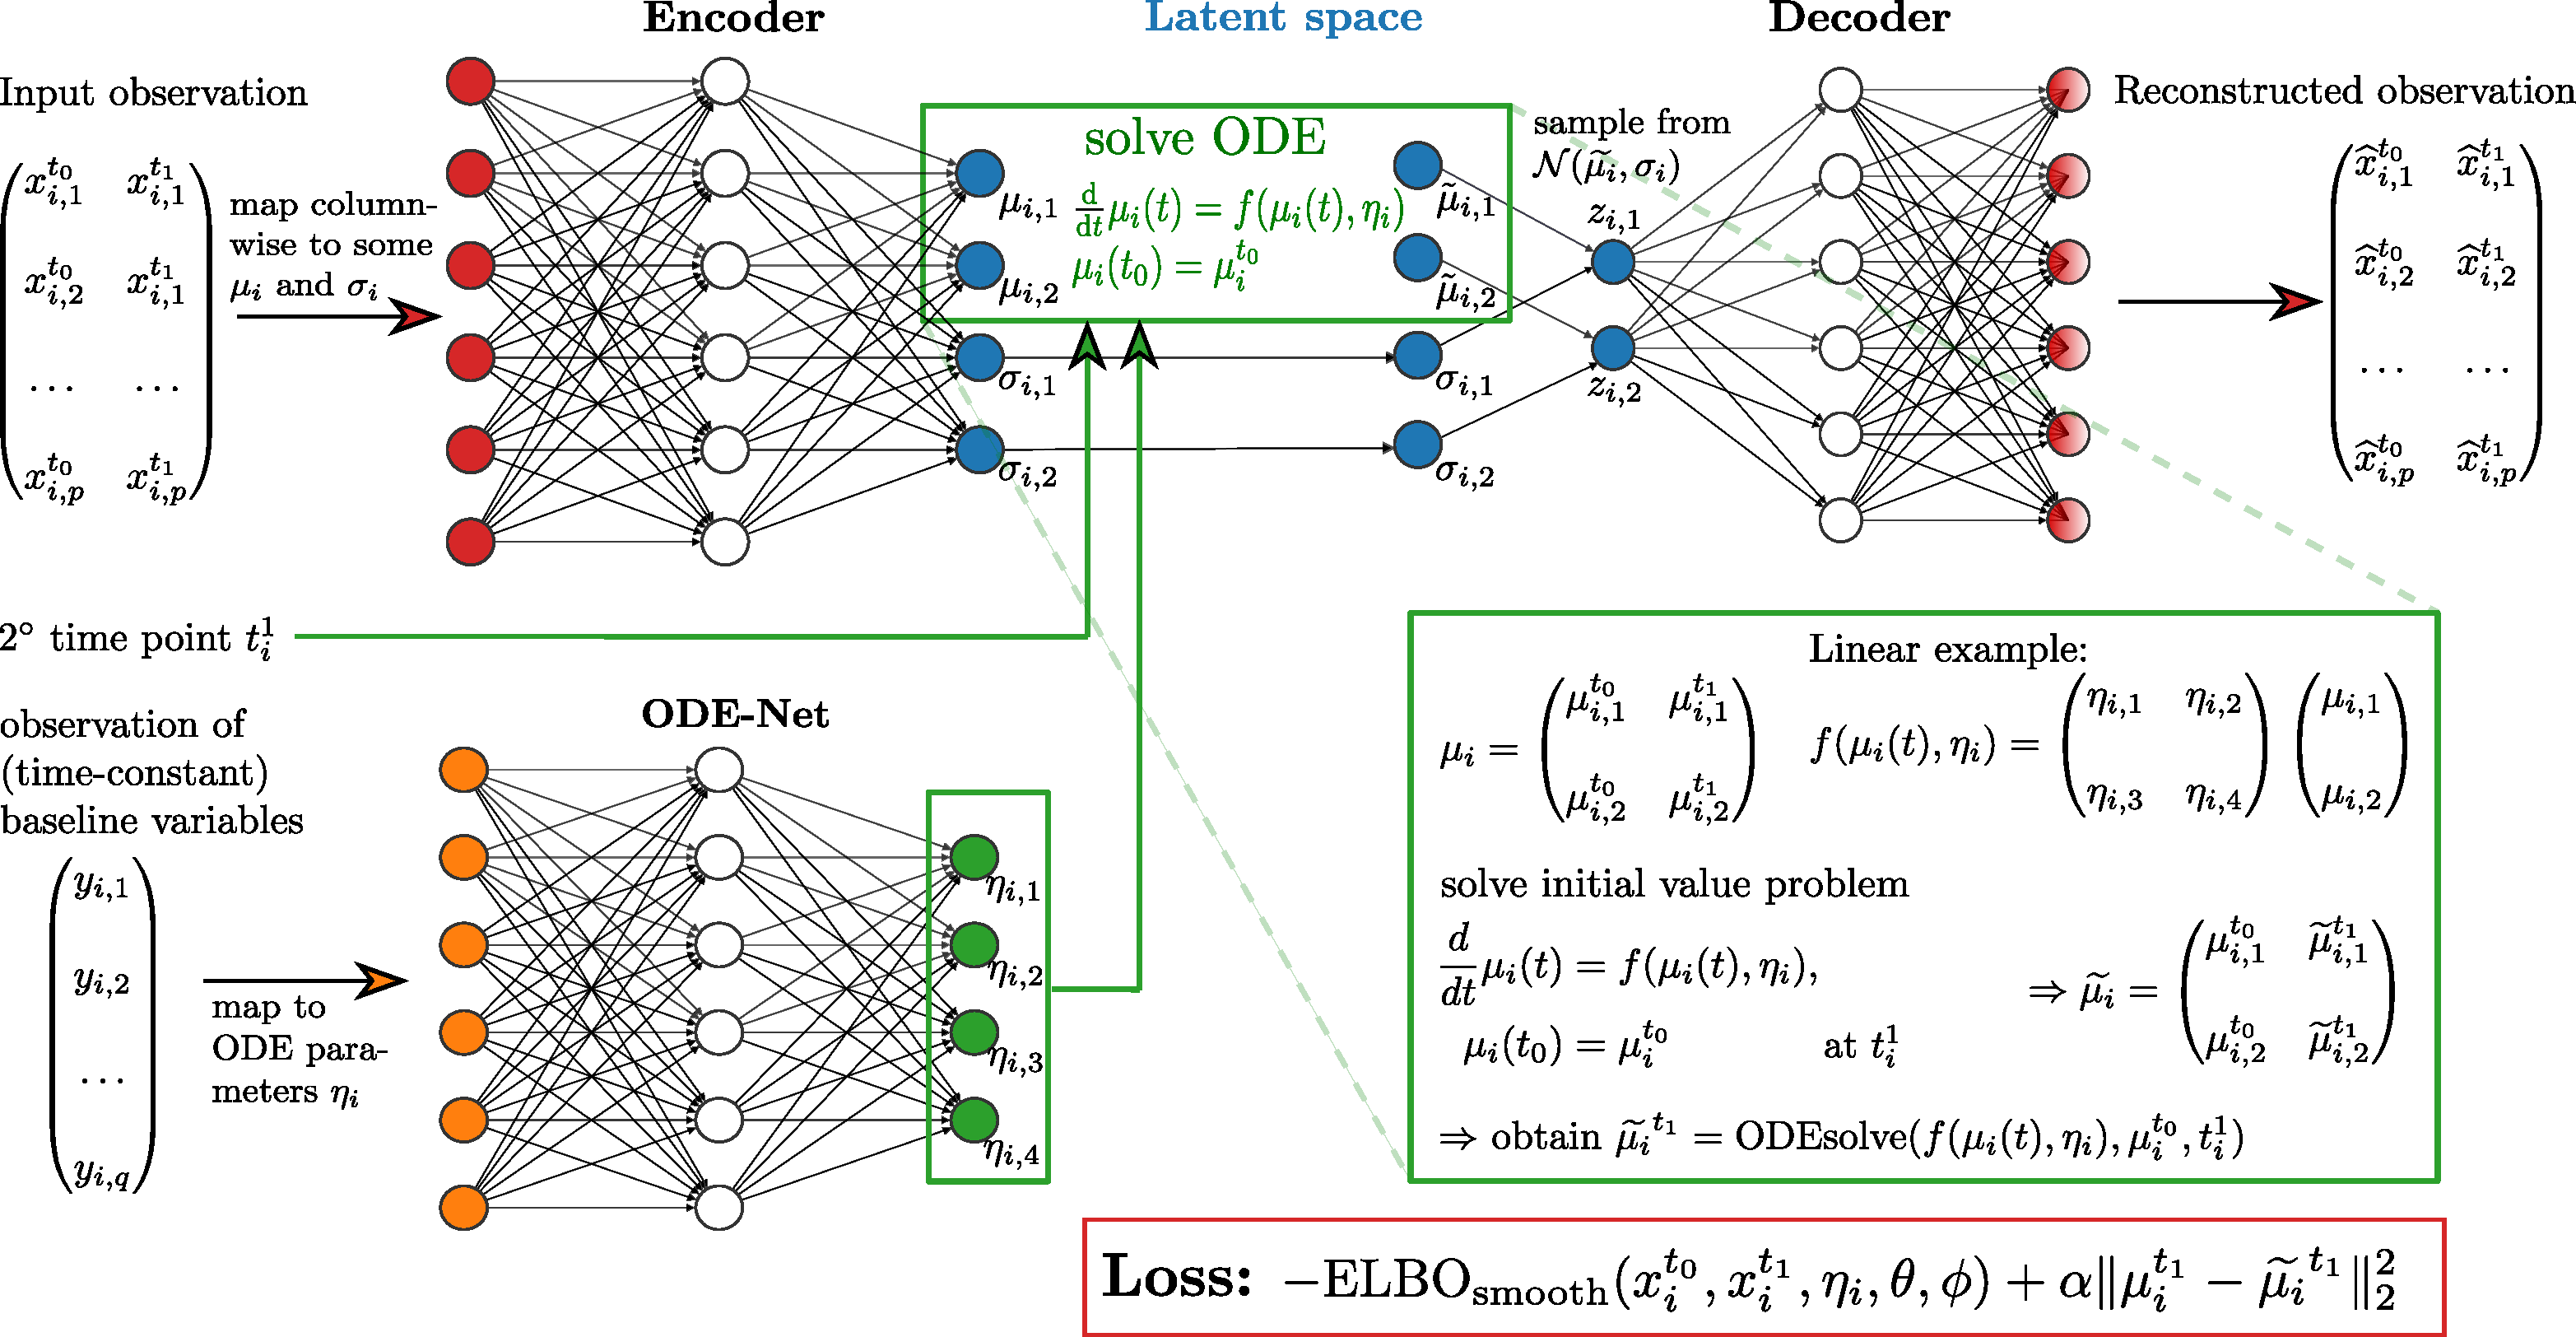
\includegraphics[width=\linewidth]{ODE_VAE_archichtecture.pdf}
	\caption{Overview of model architecture and training.}
	\label{fig:node_vae_architecture_draft}
\end{figure}

\section{Model extension: training on batches of similar individuals}\label{sec:methods-minibatches}

\subsection{Time sparsity and notion of similarity}\label{sec:methods-batches-generalintro}

A major challenge for my approach of modelling dynamic processes with individual-specific ODE systems in latent space is the strong sparsity and irregularity of the time grid with only two observations for every individual, which implies constraints on the complexity of ODE systems that can be fitted with these data. While it is natural to assume that two time points allow to estimate two unknown ODE parameters for each individual, the model should optimally also capture more complex development patterns.
% with our model and to include more parameters in the ODE systems. 
%In our applications, however, we noted that if the number of parameters exceeds the number of time points each individual is observed at, the systems are underdetermined and the model does not pick up on individual development patterns any more. 
%Their combination of all second time point measurements in the batch then serves as proxy information on the common dynamics at multiple time points,

This is achieved with an extension of my method: To every individual, a batch of individuals with similar underlying development patterns is assigned. Then, the combination of all their second time point measurements can be used as proxy information on the common dynamics at multiple time points. Thus, each observation is enriched with a group of similar ones observed at different time points and the irregularity of the time grid is exploited to address the problem of strong time sparsity, which ultimately allows to model more complex development patterns. 

More specifically, first a measure of similarity has to be defined to identify individuals with similar development patterns. Since each individual is observed at a different second time point, their measurements cannot be directly compared in data space. Additionally, if the random measurement noise in the observations superimposes the true underlying developments, it can be impossible to identify similar trajectories from the data alone.

Figure~\ref{fig:minibatches_explanation} provides an illustration of the batch assignment: For each individual, the observations are generated from one of two different underlying development patterns with a moderate level of noise. The original underlying pattern is indicated by the frame colour of each panel (violet/green). The development of the individual at the top is different from the left one in the second row, but similar to the right one in the third row.
However, it is challenging to judge from these observations alone whether the right individual in the second row and the left in the third row are based on different underlying development patterns. This becomes clear only after passing each observation through the encoder and comparing the latent representation of the trajectories: In latent space, depicted in the middle part of the figure, we can clearly distinguish the two general development patterns. 

Consequently, I define the similarity of individuals based on their latent trajectories represented by the solution of each individual's ODE system in latent space. To infer for a given individual a batch of similar ones, I therefore first pass all observations through the VAE encoder. In the latent space of ODE solutions, I calculate the $L^2$-norm of distances of the ODE solutions and sort individuals according to distance to the reference individual. 
Additionally, I use a kernel to weigh the individuals with respect to their similarity to the reference individual. The complete method is formalised in the following sections.

\begin{figure}
	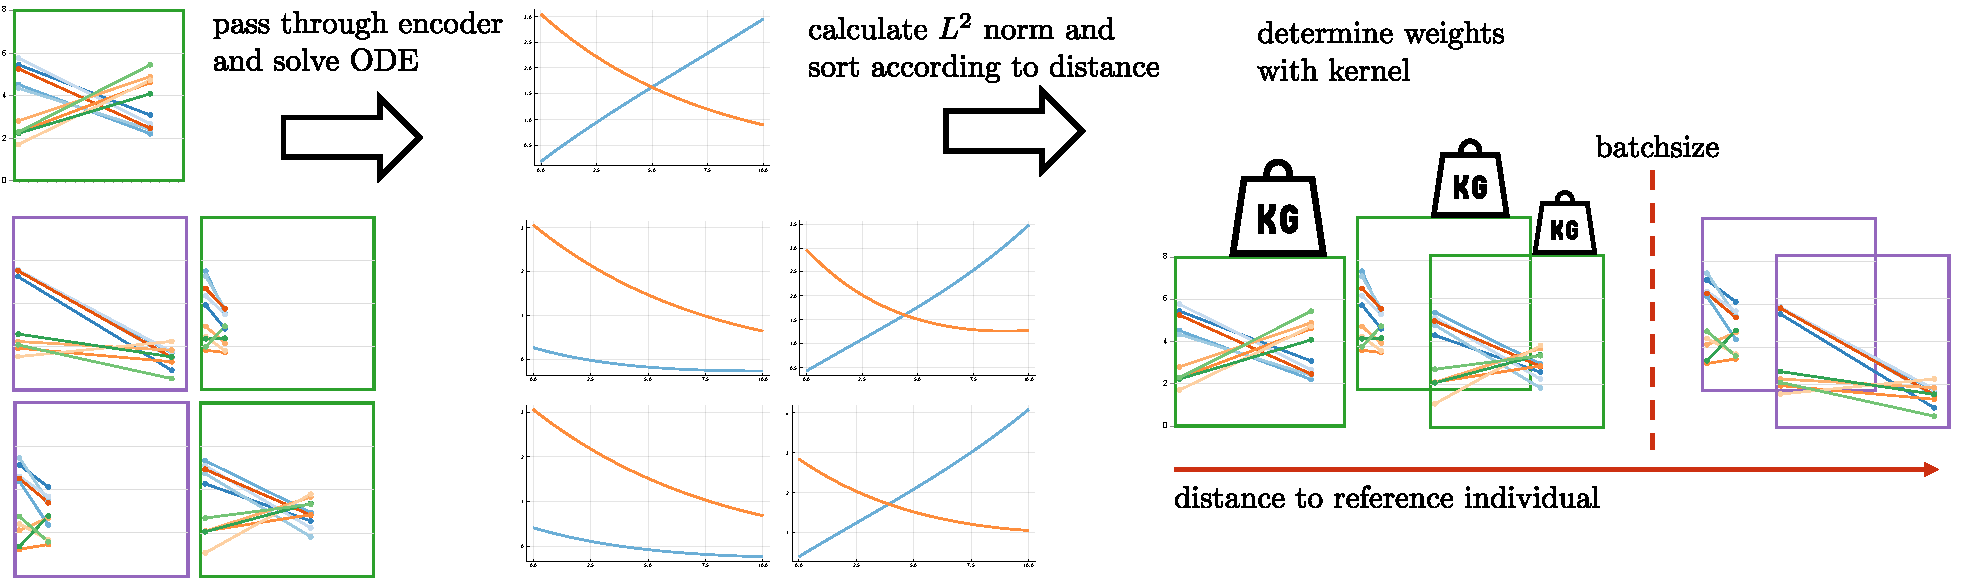
\includegraphics[width=\linewidth]{minibatches_explanation_figure_thesis.pdf}
	\caption{Assigning to an individual a batch of similar ones.}
	\label{fig:minibatches_explanation}
\end{figure}

\subsection{Defining an iterative optimisation framework}\label{sec:methods-batches-EMprocedure}

The proposed notion of similarity between individuals refers to the similarity not of their observed measurements, but of their unobserved latent trajectories, i.e., their ODE solutions in the latent space of the ODE-VAE model, that should ideally reflect the true underlying development patterns. However, inferring such a latent representation that recovers the true ODE system underlying every individual's observed measurements is the objective of the training process that we aim to improved by using the batches of similar individuals in the first place. 
In other words, a notion of similarity based on the underlying trajectories is needed to group individuals to train the model, i.e., to find a latent representation recovering the true dynamics, but at the same time such a meaningful latent representation is already needed to accurately infer individuals' similarity. 

To overcome this problem, I introduce an iterative optimisation framework that alternates between the assignment of batches of similar individuals and the joint training of the ODE-VAE model.
In this way, the latent representation of the trajectories are improved iteratively, so that they more closely reflect the true developments and individuals can be grouped more accurately based on these trajectories. Training on these groups -- that more accurately capture the similarity of the underlying patterns -- in turn improves individuals' latent representations due to better proxy information at other time points from the batch. This results in an overall training method that resembles an expectation-maximisation framework (Chapter~\ref{chap:background}, Section~\ref{sec:bayesian_inference}).\\ 

\subsubsection{Assigning a batch to each individual}

To group individuals in batches based on the similarity of their ODE solutions in latent space, every individual observation $x_i\in \mathcal{D}, i\in\lbrace1,\dots, n\rbrace$ is first passed through the VAE encoder to obtain an approximate posterior mean $\mu_i= (\mu_i\tn \quad \mu_i\te) \in \R^{k\times 2}$ and variance $\sigma_i = (\sigma_i\tn \quad \sigma_i\te) \in \R^{k\times 2}$ as in Section~\ref{sec:methods-ODE-VAEtraining}. Also, the respective baseline measurements $y_i$ are passed through the ODE-net to obtain a set of individual ODE parameters $\eta_i$. Next, each individual's ODE system as defined by the function $f$ denoting the common ODE structure and the individual parameters $\eta_i$ is solved to obtain for each individual the posterior mean according to smooth dynamics as a function of $t$:
$$\mu_i(t) = \mathrm{ODEsolve}(f(\mu_i(t), t, \eta_i)).$$
For a $T \in \R$, it holds that for all $i$, $\mu_{i} \in L^2([t_0,T])$. Now, we calculate a symmetric distance matrix 
$$D= (d_{i,j})_{i,j=1,\dots,n} = \left(\Vert \mu_i - \mu_j\Vert_{L^2([t_0,T])}\right)_{i,j=1,\dots,n}$$ 
where the $i,j$-th entry denotes the distance in $L^2$-norm between the ODE solutions $\mu_i(t)$ and $\mu_j(t)$ of individuals $i$ and $j$. In my implementation, the ODE solutions are evaluated at a fixed grid of $m+1$ time points $t_0,\dots, t_m$ to approximate the $L^2$-integral:
\begin{equation}\label{eq:discretisationl2norm}
	d_{i,j} = \left( \frac{1}{m} \sum_{t=t_0}^{t_m} \Vert \mu_i(t) - \mu_j(t)\Vert_2^2 \right)^{\frac{1}{2}}.
\end{equation}
For a pre-defined batch size of $b$, to each individual the $(b-1)$ individuals closest to that reference individual are assigned: 
Let $i\in\lbrace1,\dots, n\rbrace$ be the index of the reference individual. Of course, $d_{i,i}= 0$. The remaining entries in row $i$ are sorted such that $d_{i,j_1} \leq d_{i,j_2} \leq \dots \leq d_{i,j_{n-1}}$ where $j_k \in \lbrace 1,\dots , i-1, i+1, \dots, n\rbrace$ for $k=1,\dots, n-1$. 
For any $a <n$, the indices $j_1,\dots, j_a$ now denote the indices of the $a$ closest individuals to the reference individual. Thus, a batch $B_i$ of the $b-1$ individuals closest to $x_i$ can be defined by setting 
$$
B_i = \lbrace x_i, x_{j_1},\dots, x_{j_{b-1}} \rbrace.
$$ 
The closer an individual is to the reference individual, the more similar is its underlying development pattern. This implies that also the substistute information provided by that individual is potentially more accurate and should thus be regarded as more important for the training of the specific batch. To account for that, each individual in the batch is weighted according to its calculated distance to the reference individual. Specifically, weights $w_i, w_{j_1},\dots, w_{j_{b-1}}$ are determined for each individual in the batch $B_i$ with a smoothing kernel $K_h$, such that 
\begin{equation}\label{kernel-weights}
	w_k = \frac{K_h(d_{i,k})}{\sum_{k=i,j_1,\dots, j_{b-1}} K_h(d_{i,k})} \quad \text{for all } k=i,j_1,\dots, j_{b-1}. 
\end{equation}
The kernel is defined as the tricube function given by
$$
K(x) = \begin{cases}
(1-\mid x\mid^3)^3 & \mid x\mid \leq 1, \\
0 & \ \mathrm{else}
\end{cases}
$$
and can be scaled with the bandwidth parameter $h$ by defining  $K_h(x) = \frac{1}{h} K(\frac{x}{h})$. 

\subsubsection{Adapting the ODE-VAE loss to training on batches}

Having determined for each individual a batch of individuals exhibiting similar temporal development patterns, the ODE-VAE model is trained on the resulting batches in order to improve the estimates of the variational parameters of the approximate posterior $\phi$, the model parameters $\theta$ and the individual ODE parameters $\eta_i$ with respect to the training objective $\mathcal{L}(x_i\tn, x_i\te, \eta_i,\theta,\phi)$ of (\ref{finalELBO}): 

For each individual in the batch, the respective loss value is calculated as described in Section~\ref{sec:methods-ODE-VAEtraining}. 
Since for each individual the solution at the individual-specific second measurement time point is used to calculate its loss, those additional values now serve as proxy information for measurements at more time points (one from each individual in the batch) of the reference individual. To use them to enrich this reference individual's information and stabilise the gradient of its loss function, we derive a common loss value for the entire batch as the weighted average of individual loss values, using the weights derived from the distance matrix of the first step. The final training objective is thus given by the loss of each batch $B_i$, $i=1,\dots, n$: 
\begin{equation}\label{batches-finalcommonloss}
	\mathcal{L}_{\mathrm{batch}}(B_i, (\eta_k)_{k=i,j_1,\dots, j_{b-1}}, \theta,\phi) = \sum_{k=i,j_1,\dots, j_{b-1}} w_k \cdot \mathcal{L}(x_k\tn, x_k\te, \eta_k,\theta,\phi).
\end{equation} 

The weighting approach ensures that the individuals contributing most strongly to the common loss are the ones which best match the trajectory of the reference individual and therefore provide a good proxy for the observations of the reference individual at additional time points. 

The overall method to train the ODE-VAE model on batches now consists of iteratively applying the two steps and is summarised in Algorithm~\ref{algo-batches}.

\begin{algorithm}
	\SetAlgoLined
	\KwData{ \\ Dataset $\mathcal{D} = \lbrace x_1,\dots, x_n\rbrace$ of time-dependent variables, \\ additional baseline variables $y_1,\dots, y_n$ \\ 
		Inference model: family of approximate variational posterior distributions $(Q_{\phi}^{Z\mid x})_{\phi \in \Phi} = (\mathcal{N}(\mu,\sigma^2))_{(\mu,\sigma^2)\in\R^{k\times 2}\times \R^{k\times 2}}$, \\
		Generative model: family of joint distributions $(P_{\theta}^{X,Z})_{\theta\in \Theta}$, \\
		Function $f: \R^k \times \R \times \R^l \to \R^k$ defining general structure of latent ODE system, parameterised by $\eta \in \R^l$ }
	\KwResult{ \\ Learned parameters $(\theta, \phi)$ of the generative and inference model, individual-specific ODE parameters $\eta_i$}
	
	$(\theta, \phi, \mathrm{ODEnet} )\leftarrow$ Random initialization\;
	\While{SGD not converged}{
		\For{each datapoint $x_i \in\mathcal{D}$}{
			Compute $\eta_i = \mathrm{ODEnet}(y_i)$ \;
			Compute $\mu_i(t) = \mathrm{ODEsolve}(f(\mu(t),t,\eta_i),\mu_i\tn)$ \;
			Compute distance matrix $D = (\Vert \mu_i(t) - \mu_j(t)\Vert_{L^2})_{i,j=1,\dots, n}$ \;
			Sort $d_{i,j_1} \leq d_{i,j_2} \leq \dots \leq d_{i,j_{n-1}}$, $j_k \in \lbrace 1,\dots , i-1, i+1, \dots, n\rbrace$\;
			Define $B_i = \lbrace x_i, x_{j_1},\dots, x_{j_{b-1}} \rbrace$\; 
			Calculate $w_k = \frac{K_h(d_{i,k})}{\sum_{k=i,j_1,\dots, j_{b-1}} K_h(d_{i,k})}$\;
		}
		\For{each batch $B_i = \lbrace x_i, x_{j_1},\dots, x_{j_{b-1}} \rbrace$}{
			\For{each $x\in B_i$}{
			Sample random noise $\varepsilon \sim \P^{\mathcal{E}}$ and compute $z = g(\varepsilon, \phi, x)$\;
			Compute $\mathcal{L}(x_k\tn, x_k\te, \eta_k,\theta,\phi)$\;}
			Compute $\mathcal{L}_{\mathrm{batch}}(B_i, (\eta_k)_{k=i,j_1,\dots, j_{b-1}}, \theta,\phi) = \sum_{k=i,j_1,\dots, j_{b-1}} w_k \cdot \mathcal{L}(x_k\tn, x_k\te, \eta_k,\theta,\phi)$\;}
		Update parameters $\theta, \phi$ and ODE-net using SGD optimiser\;
	}
	\caption{Training procedure of the ODE-VAE on batches}
	\label{algo-batches}
\end{algorithm}